\documentclass[]{article}
\usepackage{lmodern}
\usepackage{amssymb,amsmath}
\usepackage{ifxetex,ifluatex}
\usepackage{fixltx2e} % provides \textsubscript
\ifnum 0\ifxetex 1\fi\ifluatex 1\fi=0 % if pdftex
  \usepackage[T1]{fontenc}
  \usepackage[utf8]{inputenc}
\else % if luatex or xelatex
  \ifxetex
    \usepackage{mathspec}
  \else
    \usepackage{fontspec}
  \fi
  \defaultfontfeatures{Ligatures=TeX,Scale=MatchLowercase}
\fi
% use upquote if available, for straight quotes in verbatim environments
\IfFileExists{upquote.sty}{\usepackage{upquote}}{}
% use microtype if available
\IfFileExists{microtype.sty}{%
\usepackage{microtype}
\UseMicrotypeSet[protrusion]{basicmath} % disable protrusion for tt fonts
}{}
\usepackage[margin=1in]{geometry}
\usepackage{hyperref}
\hypersetup{unicode=true,
            pdftitle={Age-related gene expression variations reak in human monocytes and T cells},
            pdfauthor={C. Valencia},
            pdfborder={0 0 0},
            breaklinks=true}
\urlstyle{same}  % don't use monospace font for urls
\usepackage{graphicx,grffile}
\makeatletter
\def\maxwidth{\ifdim\Gin@nat@width>\linewidth\linewidth\else\Gin@nat@width\fi}
\def\maxheight{\ifdim\Gin@nat@height>\textheight\textheight\else\Gin@nat@height\fi}
\makeatother
% Scale images if necessary, so that they will not overflow the page
% margins by default, and it is still possible to overwrite the defaults
% using explicit options in \includegraphics[width, height, ...]{}
\setkeys{Gin}{width=\maxwidth,height=\maxheight,keepaspectratio}
\IfFileExists{parskip.sty}{%
\usepackage{parskip}
}{% else
\setlength{\parindent}{0pt}
\setlength{\parskip}{6pt plus 2pt minus 1pt}
}
\setlength{\emergencystretch}{3em}  % prevent overfull lines
\providecommand{\tightlist}{%
  \setlength{\itemsep}{0pt}\setlength{\parskip}{0pt}}
\setcounter{secnumdepth}{0}
% Redefines (sub)paragraphs to behave more like sections
\ifx\paragraph\undefined\else
\let\oldparagraph\paragraph
\renewcommand{\paragraph}[1]{\oldparagraph{#1}\mbox{}}
\fi
\ifx\subparagraph\undefined\else
\let\oldsubparagraph\subparagraph
\renewcommand{\subparagraph}[1]{\oldsubparagraph{#1}\mbox{}}
\fi

%%% Use protect on footnotes to avoid problems with footnotes in titles
\let\rmarkdownfootnote\footnote%
\def\footnote{\protect\rmarkdownfootnote}

%%% Change title format to be more compact
\usepackage{titling}

% Create subtitle command for use in maketitle
\newcommand{\subtitle}[1]{
  \posttitle{
    \begin{center}\large#1\end{center}
    }
}

\setlength{\droptitle}{-2em}
  \title{Age-related gene expression variations reak in human monocytes and T
cells}
  \pretitle{\vspace{\droptitle}\centering\huge}
  \posttitle{\par}
\subtitle{140.688.01 - Statistics for Genomics}
  \author{C. Valencia}
  \preauthor{\centering\large\emph}
  \postauthor{\par}
  \predate{\centering\large\emph}
  \postdate{\par}
  \date{`r Sys.Data()'}


\begin{document}
\maketitle

\hypertarget{introduction}{%
\subsection{Introduction}\label{introduction}}

The Multi-Ethnic Study of Atheroesclerosis (MESA) in an ongoing study of
\textasciitilde{}6000 men and woman from six communities in the United
States. The MESA Epigenomics and Transcriptomics Study is an ancillary
study that aims to investigate potential difference in gene expression
and methylation across age. For the purpose of the present analysis we
will focus only on the gene expression data. A total of 214 individuals
were randomly selected for T cell isolation. Also \textasciitilde{}1200
random individuals were also selected for monocyte isolation.

We aim to study genes differentially express by age accounting by sex
using the two cell types however, we notice two main problems:

\begin{itemize}
\tightlist
\item
  Variable sex does not appear in the phenotype data
\item
  There was not clear way to match ID between the monocyte dataset and
  Tcell dataset
\end{itemize}

To solve this problem we decide to predict sex using gene expression
data and then use this predicted sex in the differential expression
analysis. Also, we decided to conduct a two factor matching approach to
select the same individuals from both datasets.

\hypertarget{processing}{%
\subsection{Processing}\label{processing}}

The expression data was Illumina HumanHT-12 V4.0 expression beadchip and
it was processed using the limma package.

We removed bad quality probes (12375), and then predict sex using the
probes from the Y chromosome with a high variance (92). There were 97
predicted female and 117 predicted males.

We then proceeded with the differential expression analysis by cell
type. We started by looking at gene differentially express across age
span (model 1) then we will include sex (model 2) and finally we will
caterorize age by the median (58 years) and add sex into the model
(model 3)

\includegraphics{./Vplot.mod1.pdf} \includegraphics{./Vplot.mod2.pdf}
\includegraphics{./Vplot.mod3.pdf}

\hypertarget{monocytes}{%
\subsection{Monocytes}\label{monocytes}}

Finally, we also look at genes differentially express across age span in
monocytes

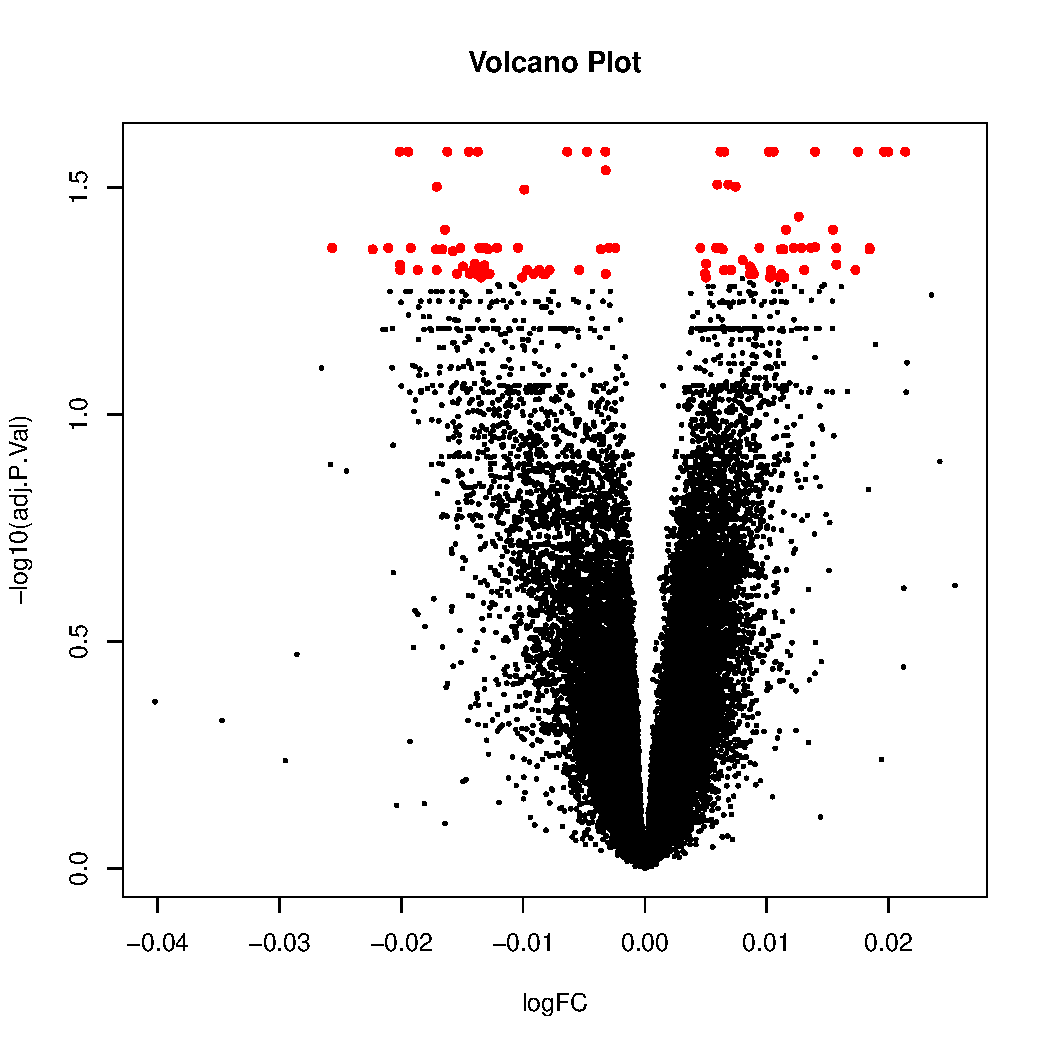
\includegraphics{./Vplot.Mod1_Mono_ageContinuous.pdf}
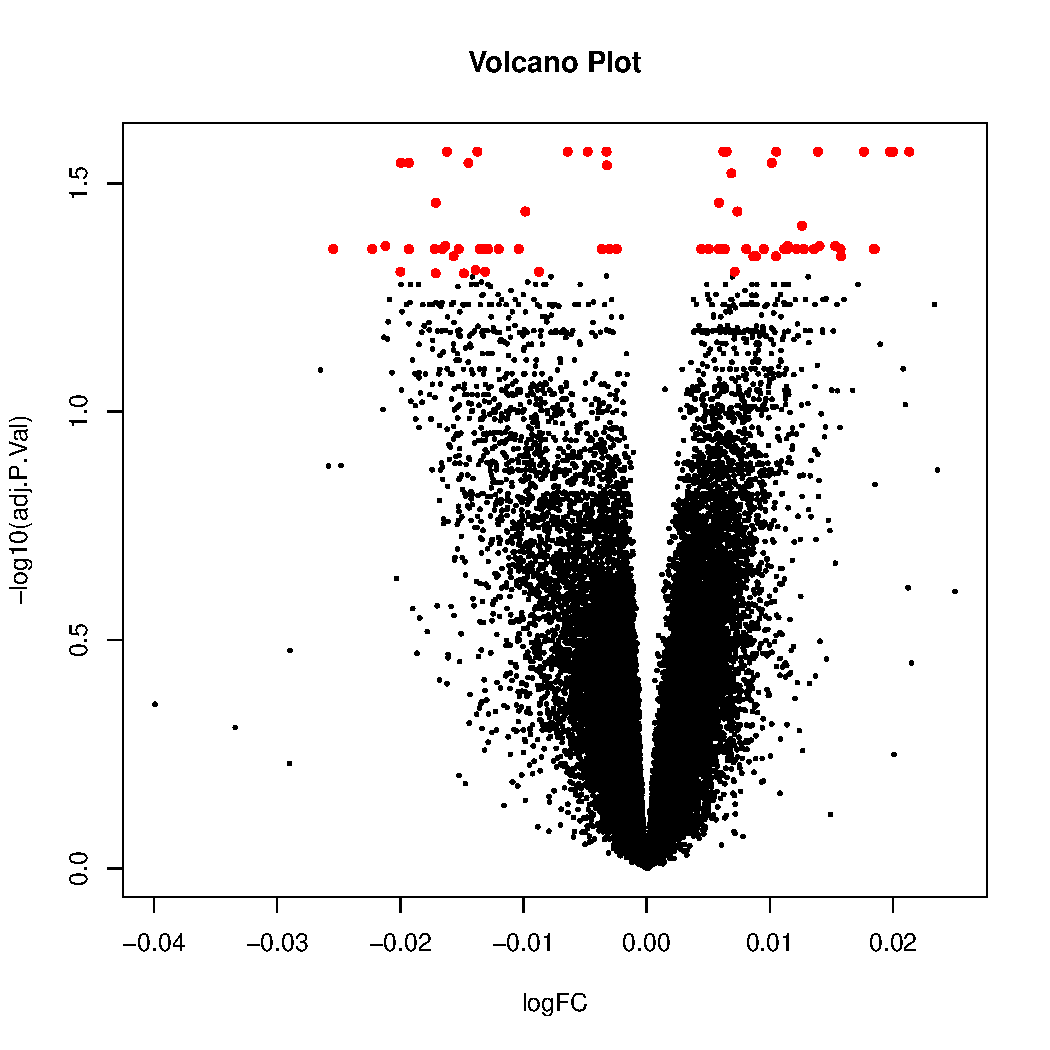
\includegraphics{./Vplot.Mod2_Mono_ageContinuous_sex.pdf}
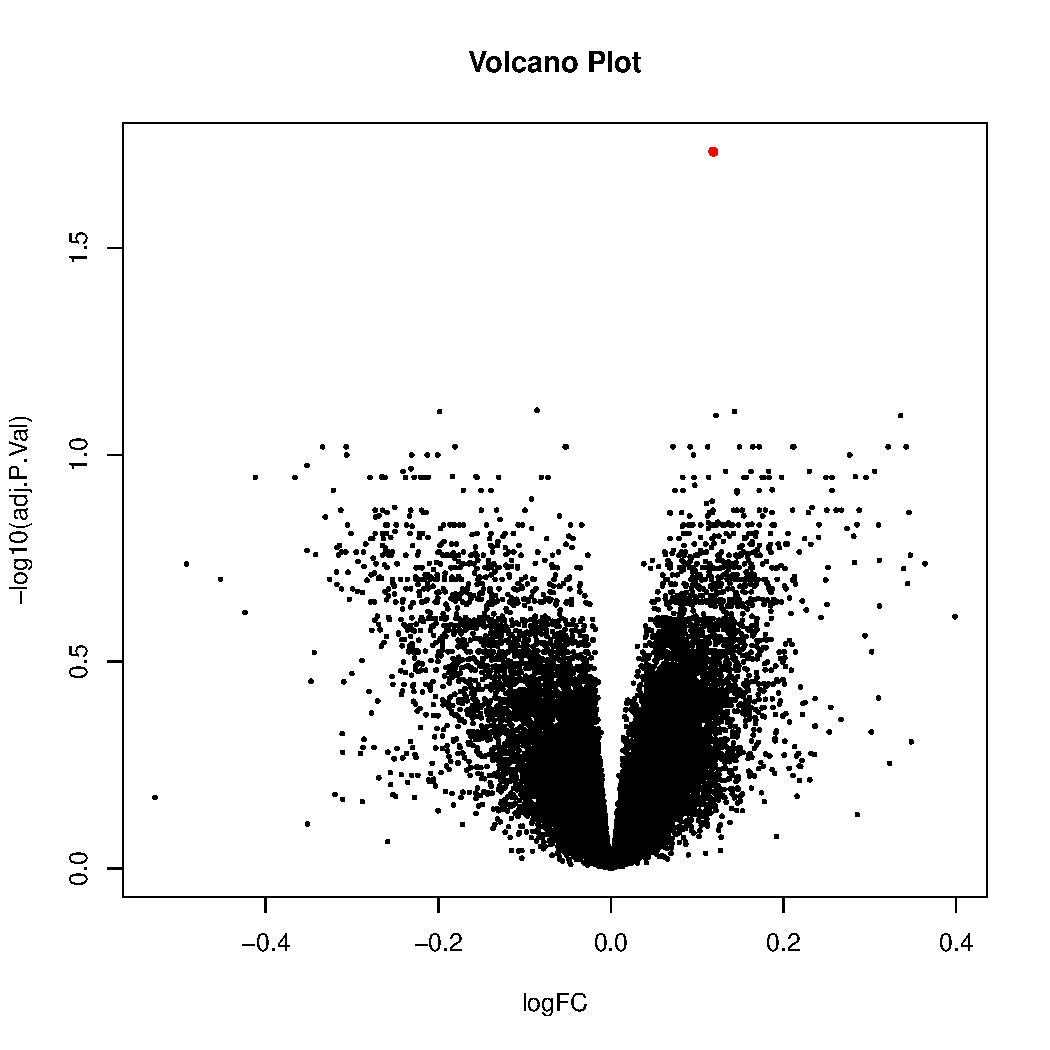
\includegraphics{./Vplot.Mod3_Mono_ageCategorical_sex.pdf}

\hypertarget{conclusion}{%
\subsection{Conclusion}\label{conclusion}}

\begin{itemize}
\tightlist
\item
  We were able to predict sex using expression data.
\item
  There were differentially express genes by age and sex in monocytes
  however this difference were minor or not observed in CD4 T cells.
\end{itemize}


\end{document}
